\documentclass[10pt]{article}
\usepackage{amsmath}
\usepackage{amssymb}
\usepackage{amsthm  }
\usepackage{fancyhdr}
\usepackage[margin=0.5in]{geometry}
\usepackage{graphicx}
\usepackage[utf8]{inputenc}
\usepackage{listings}
\usepackage{pdfpages}
\usepackage{standalone}
\usepackage{titling}
\usepackage{braket}
\usepackage{color}
\usepackage{hyperref}
\usepackage{wrapfig}
\usepackage{float}


\definecolor{dkgreen}{rgb}{0,0.6,0}
\definecolor{gray}{rgb}{0.5,0.5,0.5}
\definecolor{mauve}{rgb}{0.58,0,0.82}
\lstset{
  language=C,
  aboveskip=3mm,
  belowskip=3mm,
  showstringspaces=false,
  columns=flexible,
  basicstyle={\small\ttfamily},
  numbers=none,
  numberstyle=\tiny\color{gray},
  keywordstyle=\color{blue},
  commentstyle=\color{dkgreen},
  stringstyle=\color{mauve},
  breaklines=true,
  breakatwhitespace=true,
  tabsize=4
}

\newcommand{\NN}{\mathbb{N}} % Naturals
\newcommand{\ZZ}{\mathbb{Z}} % Integers
\newcommand{\QQ}{\mathbb{Q}} % Rationals
\newcommand{\RR}{\mathbb{R}} % Reals
\newcommand{\CC}{\mathbb{C}} % Imaginaries
\newcommand{\HH}{\mathbb{H}} % Quaternions
\newcommand{\FF}{\mathbb{F}} % Field

\newcommand{\ud}{\,\mathrm{d}} % Single-var differential (use like \partial)

\newcommand{\CoulombConstant}{\frac{1}{4\pi\epsilon_0}}

\DeclareMathOperator{\erf}{erf} % Error Function
\DeclareMathOperator{\erfc}{erfc} % Complementary Error Function
\DeclareMathOperator{\erfi}{erfi} % Imaginary Error Function
\DeclareMathOperator{\row}{row} % Matrix Row
\DeclareMathOperator{\col}{col} % Matrix Column
\DeclareMathOperator{\trace}{tr} % Matrix Trace
\DeclareMathOperator{\proj}{proj} % Vector Projection

\title{PHYS 319 Final Project: PWM-Based Synthesizer}
\author{Ashtan Mistal}
\date{April 2022}

\begin{document}

\maketitle

\break

\tableofcontents{}

\break

% TODO:
% - finish abstract
% - edit introduction
% - Measure input on a FFT on Studio One (a spectral filter may be more accurate)
% - Compare to proper square wave
% - accuracy of the square wave frequency using a tuner
% - add conclusion
% - finish theory for tjhe ADSR envelope
% - add appendix for the ADSR envelope code
% - add appendix for the square wave code (PWM code)
% - finish Table of Notes to Frequency Values appendix
% - make circuit diagrams for current project and previous rendition
% - add bibliography


\section{Abstract}\label{sec:abstract}

% [abstract here]

\section{Introduction}\label{sec:introduction}

% [introduction here]
Exploration into the possibility of creating a user-controlled, MIDI\footnote{musical instrument digital interface}-compatible fully featured synthesizer has held a personal interest shortly after I became interested in music production itself.
Motivation for this project to encompass this personal interest stemmed from first using pulse width modulation to change the brightness of a bulb during an earlier lab.
Since my more recent interest in audio equipment itself, I was motivated to do an audio-related project.
The purpose of this project, as a result, was to help me gain a further understanding into the inner workings of oscillators and envelope generators, gain an appreciation for the MIDI standard, and of course to have a working, hand-made synthesizer for future music production related use.
All three areas of knowledge mentioned above would aid in future audio-related projects, both in software as well as in hardware, and help inspire for future related projects.
This project builds off of my previous related experience in music production, which provided me with a background on audio synthesis and processing.

\section{Theory}\label{sec:theory}
% A presentation of the theoretical background necessary to understand your project. Not every project will need a theory section, but most will. Here you would describe the physics of how sensors you use work (eg how does accelerometer measure acceleration, or how does a capacitive touch sensor work), or how an electrical interface to a device works.

\subsection{Digital - Analog Converter}\label{subsec:digital---analog-converter}

The primary goal of a digital to analog converter is to convert data bits (strictly HIGH or LOW), and convert to an analog signal with voltage varying on the values of the data bits.
This can be done either by receiving all data pins at once, or sending the data pins individually along with a clock bit, which is then read by a segment in the integrated circuit that decodes the data.
Receiving all data pins at once does not require the use of an integrated circuit, and can be done using resistor ladders.
More details regarding resistor ladders will be shown below.
Nonetheless, the DAC allows us to input a certain number of bits, in the case of this project, 10 bits, and convert to an analog signal (thereby giving us 1024 different values from 0 volts up until the maximum voltage).
This is essentially "receiving what output voltage to emit in binary", so that 1111111111, all pins on, corresponds to the maximum voltage, and 0000000000 (all pins off) correspond to minimum voltage, and something like 1101100110 till be $\frac{870}{1023}$ of the maximum. 

\subsection{Analog - Digital Converter}\label{subsec:analog---digital-converter}

an analog to digital works in the exact opposite way as a digital to analog converter.
By taking in an input voltage (as a proportion of the maximum voltage), an analog to digital converter will set some data value to be equal to that input voltage as a binary proportion to the maximum (or reference) voltage.
In the case of the microprocessor, this will be 3.3 volts.
The usage of this in the project is to be able to perform certain actions based on the value of this input pin, i.e. control the frequency based on what notes are being pressed. 

\subsection{Low Pass Filter}\label{subsec:low-pass-filter}

The theory behind an analog low pass filter is relatively simple;
the signal is sent through an RC circuit (see figure~\ref{fig:LPF}), which, due to the charging and discharging properties of a capacitor, allows us to block frequencies past a certain cutoff frequency.
This cutoff frequency is given by the following formula:

\[
f_{cutoff}=\frac{1}{2 \pi R C}
\]

So, in order to reduce unnecessary signal noise, we can apply a low pass filter to block frequencies past the human range of hearing, as well as attenuate higher pitched distortion coming from the circuit. 

In the specific case of this project, a 9.55 nF capacitor was made available.
Using the formula mentioned above, we can set the cutoff frequency to 20 kHz, therefore using a resistor of 800 Ohms. 

\begin{figure}[H]
    \centering
    \includegraphics[width = 0.4 \textwidth]{lowpassfilter}
    \caption{A basic circuit diagram of a low pass filter. } % cite here
    % https://www.allaboutcircuits.com/technical-articles/low-pass-filter-tutorial-basics-passive-RC-filter/
    \label{fig:LPF}
\end{figure}

We can graph what the resultant signal graph will be post-LPF by using the following formula. This formula is derived from the formula for a voltage divider circuit. 



\[
V_{out}=V_{in}\left(\frac{X_{C}}{\sqrt{R_{1}^{2}+X_{C}^{2}}}\right)
\]

where

\[
X_{C}=\frac{1}{2 \pi f C}
\]

Hence, assuming $V_{in}$ is kept constant at 3.3 volts, we can view the output voltage as a function of the frequency, with $C = 9.55*10^{-9}$ F, and $R_1 = 800 \Omega$. 

\begin{figure}[H]
    \centering
    \includegraphics[width = 0.5 \textwidth]{lpfgraph}
    \caption{Plot of voltage versus frequency (linear scale) for an RC low pass filter. }
    \label{fig:lpfgraph}
\end{figure}

\subsection{MIDI Standard}\label{subsec:midi-standard-theory}
% https://www.instructables.com/Send-and-Receive-MIDI-with-Arduino/

Next, we delve further into details regarding the MIDI standard.
Note that this is strictly regarding the standard, and details regarding receiving MIDI data on the microprocessor will be described in Section~\ref{subsec:previous-apparatus-renditions}.

Sending MIDI data works by sending a stream of bytes at a given baud rate\footnote{The rate at which information is transferred in a communication channel.}. %https://www.setra.com/blog/what-is-baud-rate-and-what-cable-length-is-required-1#:~:text=The%20baud%20rate%20is%20the,of%209600%20bits%20per%20second.
This data is then decoded and processed, and instrument-related actions are taken accordingly. 

MIDI data is sent in either 2 or 3 bytes of information, depending on what the first byte is.
The first byte is always a command byte:

\[
\begin{array}{l|l}
10000001 & \text { note off } \\
10010001 & \text { note on } \\
10100001 & \text { aftertouch } \\
10110001 & \text { continuous controller } \\
11000001 & \text { patch change } \\
11010001 & \text { channel pressure } \\
11100001 & \text { pitch bend } \\
11110001 & \text { non-musical commands }
\end{array}
\]

The latter half-byte in the command is what channel the command is being sent on (in this case, they are all being sent on channel 1. 

If the command is a Note On, Note Off, or aftertouch, the first byte that is sent after the command is what note was pressed, and the second is the velocity value or aftertouch value, respectively. IF the command is a controlled change or similar, the first byte that is sent after the command is what controller number was changed, and its new value. We are ignoring aftertouch, patch change, channel pressure, pitch bend, and non-musical commands in this project. 

Hence, we can read the first byte, quickly decode it, and read the second byte and third byte accordingly.
The C implementations are in Appendix~\ref{sec:-table-of-notes-to-frequency-values}.

When reading a note on / off command, the second byte corresponds to what note is being played.
There is a direct conversion from the MIDI note to the frequency, through the following formula:




\subsection{PWM-Based Synthesis}\label{subsec:pwm-based-synthesis-theory}

\subsection{Envelope Generation}\label{subsec:envelope-generation-theory}

\section{Apparatus}\label{sec:apparatus}
% Description of the project including diagrams of electrical and mechanical aspects. Depending on the complexity of the circuitry, a separate block diagram that shows functional blocks might be beneficial in addition to complete electrical schematics. The text should provide details on how the apparatus works. This section should also include a description of how your project is used.

\subsection{PWM Based Synthesis Apparatus}\label{subsec:pwm-based-synthesis-apparatus}

The actual PWM was generated on the MSP430G2553 microcontroller.
There was no need to send the signal to a DAC, as the PWM signal was directly sent to the low pass filter. 
As was discussed in Section~\ref{subsec:low-pass-filter}, the low pass filter was used to remove any unintended high frequency noise caused by the synthesizer and also to smooth out DAC volume changes. The low pass filter also allows the note OFF implementation to work: When the voltage inputted into the microprocessor was at its "default" value (both the default in the if statements in the code as well as when the voltage is at the level when no buttons are pressed), the period of the PWM was set to 2, and hence the duty cycle set to be 1. This frequency is high - 500000 Hz to be exact - and so to avoid unnecessary output interference and block short-term voltage fluctuations, this is blocked by the low pass filter. The LPF is also necessary as the MSP430 has a 32-kHz watch crystal - meaning the Nyquist frequency is 16 kHz. It may have actually been a good idea to increase the resistance such that the cutoff frequency on the LPF was below the 16 kHz mark to further avoid aliasing, but nonetheless frequencies at and above this range are still somewhat attenuated with the cutoff frequency being set to 20 kHz as we saw in Figure \ref{fig:lpfgraph}. 

This LPF was then connected to an AUX output. 
This AUX output was then connected to a speaker, however the goal of having an AUX output was to be able to connect to anything -- which is indeed the case. A speaker was used for demonstration purposes, but for measurement purposes as we see in Section \ref{sec:discussion}, this AUX output was connected to an audio interface to be able to be measured. This allowed us to analyze the signal on a computer, instead of having to use a microphone to record the signal which would lead to a less accurate representation of the signal.

The actual circuit diagram for the output is very simple (as it's just a low pass filter and a speaker), and will be included in Section~\ref{subsec:apparatus-details}.


\subsection{Apparatus Details}\label{subsec:apparatus-details}

The final rendition of this project is relatively simple in terms of electronics.
We begin by sending a signal of the same voltage to 10 different buttons, which act as the user control for the frequency of the wave emitted from the PWM\@.
The project is intended to be used similarly to a piano, with the 10 buttons available corresponding to various keys on a piano, ranging from A4 to C6, excluding sharps and flats in the note range.
When these buttons are pressed, the corresponding amplitude of the input signal is changed by sending the bits to a 10 bit DAC, which was done using a resistor ladder based on the R-2R architecture, where the resultant signal is read through a 10-bit ADC (thus allowing for the same level of precision for the DAC as is available for the ADC) that is built into the MSP430G2553 microprocessor. 
When the ADC decodes the input, the period of the PWM signal accordingly by modifying a global variable.
The duty cycle is then set to always be 50\%, by bit shifting the value of the global variable to the right by 1 bit.
Finally, the signal is outputted, and heard by the user. 

The code for this implementation is in Appendix \ref{sec:appendix-d:-pwm-synthesizer-code}. 

The circuit diagram is shown in Figure \ref{fig:circuit_diagram}. It was discovered that a USB power supply to the switches was not necessary, and the whole project could be powered by connecting the ground of the MSP430 to the switches itself as we see in the diagram. While this \textit{works}, this method may also be the rationale behind the unexpected voltage fluctuation (hence frequency fluctuation) observed in the output. It would have been a smart idea to separate the grounds and power the inputs separately. 

% include circuit diagram

\begin{figure}
    \centering
    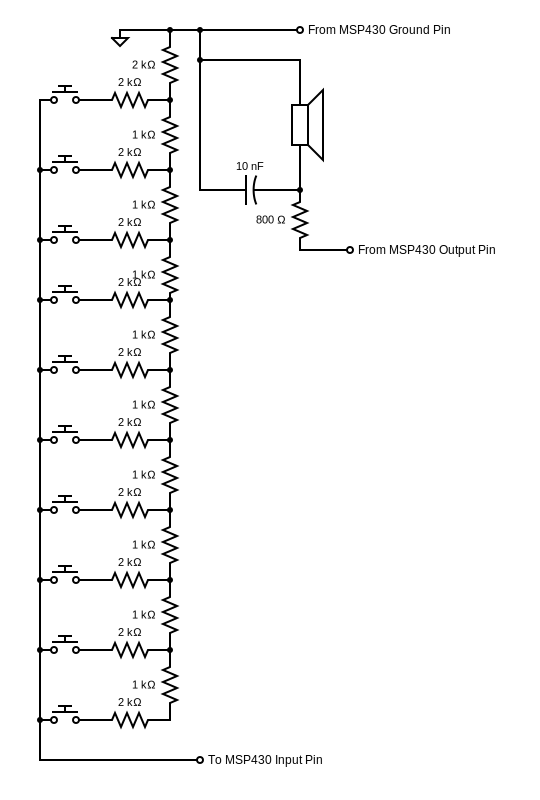
\includegraphics[width = 0.8 \textwidth]{circuit.png}
    \caption{Circuit diagram for PWM-based synthesizer. Self-powered through the MSP430. Note that the speaker is just denoting the existence of an audio output, and is actually the AUX output and not necessarily an actual speaker. }
    \label{fig:circuit_diagram}
\end{figure}






\subsection{How the project is used}\label{subsec:how-the-project-is-used}

The use of the project is relatively simple: The user plugs in the MSP430 to a power source, and plugs in headphones or a 3.5mm TRS cable to the output port. Once the synthesizer is powered on, the user plays the keys like a piano, where A4 is the leftmost key (assuming orientation of synthesizer is such that the headphone jack is facing the user, and the low pass filter is to the right of the buttons), and C6 us the uppermost key. 


\subsection{Previous Apparatus Renditions}\label{subsec:previous-apparatus-renditions}

As the initial intention of this project was to include MIDI compatibility, it is important to also include circuit diagrams for this, given it offered different methods of user interaction.
The rendition of the project that allowed for MIDI input was the 3 oscillator version (which, as will be discussed in the Results section, did not work properly due to hardware limitations).
Thus, the apparatus diagram below will reflect the legacy oscillators. The MIDI compatible circuit diagram is shown in Figure \ref{fig:3oscillatordiagram}. 

Note that the sending of the output through the 8 separate pins instead of the single output pin is due to sending the direct digital signal to an 8 bit DAC, as using just a PWM does not require the use of a DAC (unlike adding the 3 waveforms together). 
Adding the 3 waveforms together would certainly be \textit{possible} using a PWM, but would be jsut as computationally expensive. 

The reason that this circuit diagram is still being shown and discussed is because it was the original intention of the project, and is significantly more complicated, thorough, and playable than the PWM version - if it worked (limitations and reasons why are discussed in Section \ref{sec:results}. 

The MIDI was being sent by an Edirol UA 25-EX Audio Interface, controlled by Presonus Studio One. 

\begin{figure}
    \centering
    \includegraphics[width = 0.98 \textwidth]{midicircuit.png}
    \caption{Circuit diagram for the MIDI compatible, 3 oscillator version. Note that the speaker is just denoting the existence of an audio output, and is actually the AUX output and not necessarily an actual speaker.}
    \label{fig:3oscillatordiagram}
\end{figure}

\section{Results}\label{sec:results}

% How did the device perform? Did it work according to the expectations? Comparison of theory to results obtained (as quantitative as possible). Problems encountered, graph(s) of data obtained, if appropriate, accuracy of the device (if it is a measuring instrument).
Unfortunately, the 3 oscillator version did not work properly due to software limitations.
When iterating through the different waveforms, the period set in the for loop was wildly inaccurate.
This was due to the fact that this was largely hardware-based, and did not use a timer to ensure accuracy of the period being set.
Hence, the actual period was based on the number of CPU cycles that were executed, which changed based on the period due to numerous factors.

Some of these factors include the use of multiplication, division, and modulo, which were not available in the MSP430G2553 microprocessor on a hardware level and thus were computationally expensive.
Because there was this large computational overhead, not only was the waveform itself inaccurate, but the MIDI data was unable to be processed in a timely manner.
The 3 oscillator version was therefore only able to act as a noise generator, and was not able to be used as a semi-realistic synthesizer.

Nonetheless, the PWM based, single oscillator version was much more accurate than the 3 oscillator version.
The PWM based version was able to accurately reproduce a square wave with a given period, mainly due to the fact that the PWM is based on a timer, which is able to accurately set the period and is also not based on the number of CPU cycles.





\section{Discussion}\label{sec:discussion}

% Discuss what went well, and what could have been better, possible improvements to the device.

It would have been a much better idea to use 3 PWM signals instead of 3 iterative waveforms, and modify the period and duty cycle accordingly to match the given waveform being played.
This would have allowed for a much more accurate representation of the waveform being played, and would have allowed for the use of a timer to accurately set the duty cycle.
Of course, this may have had its own limitations as well, as we would have to be accurately changing the duty cycle of the PWM signal, and this would have required another timer to be used, along with numerous interrupts.
This may have been a better idea, but still is at risk of being too computationally expensive due to the constant changing of the duty cycle with a semi-unknown period (due to the fact that we have so many notes that could be played)
Early analog synthesizers combated this problem, and simultaneously allowed for polyphony, by using a separate waveform generator for each note.
But alas, this is too expensive for our microprocessor, and the 3 oscillator version was not able to be used as a real-time synthesizer, and the PWM based version was not "interesting" enough for real-world use (albeit was much more accurate and actually playable).

The primary source of inaccuracy for the PWM based version was the DAC being used to convert the notes being pressed to an analog signal.
Precision resistors were not used, and so a lot of fluctuation was observed in the analog input signal.
This is observed in the FFT signal discussed inFigure~\ref{fig:fft}.

\section{Conclusions}\label{sec:conclusions}

% Was it worth constructing? What did you learn?



%include references here
% Sources other than the course lab manual or lab web page should be referenced. Especially if your code is based on code you found on the web or elsewhere, you should make sure that the body of your report contains a clear citation to the source you used, and a corresponding reference here in the references section. In the body of the report, you should also explain clearly what differentiates your code from the source you used.

\appendix

\section{Appendix A: Table of Notes to Frequency Values}\label{sec:-table-of-notes-to-frequency-values}



% Any additional material that should be included in the report, but not necessary for the main body can be included as appendices. You should definitely include (well-annotated) program listings.

\begin{table}[h]
    \centering
    \begin{tabular}{c|c}
         &  \\
         & 
    \end{tabular}
    \caption{Table of Notes to Frequency Values}
    \label{tab:pianonotestofrequency}
\end{table}

\section{Appendix B: C Code for Decoding MIDI Data}\label{sec:appendix-b:-c-code-for-decoding-midi-data}
Please note that functions regarding the actual waveform generation were ignored here for space and organization purposes. 

\begin{lstlisting}[label={lst:lstlisting}]
//
// Created by Ashtan Mistal on 2022-03-24.
//

#include "msp430.h"
#include "msp430g2553.h"

unsigned long frequency;
unsigned long amplitude;
unsigned long noteon;
unsigned long square_wave_volume;
unsigned long noise_wave_volume;
unsigned long triangle_wave_volume;
unsigned long sawtooth_wave_volume;
unsigned long attack_rate;
unsigned long decay_rate;
unsigned long sustain_level;
unsigned long release_rate;

void send_output(int input) {
    P1OUT = input;
}

// take in MIDI note and convert to frequency
// midi note is a number between 0 and 127
int midi_to_frequency(int midi_note) {
    // this is a slow function because it declares a variable every time it is called
    // will be better to declare a global variable and use that instead
    int midi_to_frequency_table[128] = {
        8, 8, 9, 9, 10, 10, 11, 12, 12, 13, 14, 15, 16, 17, 18, 19, 20, 21, 23, 24, 25, 27, 29, 30, 32, 34, 36, 38, 41, 43, 46, 48, 51, 55, 58, 61, 65, 69, 73, 77, 82, 87, 92, 97, 103, 110, 116, 123, 130, 138, 146, 155, 164, 174, 184, 195, 207, 220, 233, 246, 261, 277, 293, 311, 329, 349, 369, 391, 415, 440, 466, 493, 523, 554, 587, 622, 659, 698, 739, 783, 830, 880, 932, 987, 1046, 1108, 1174, 1244, 1318, 1396, 1479, 1567, 1661, 1760, 1864, 1975, 2093, 2217, 2349, 2489, 2637, 2793, 2959, 3135, 3322, 3520, 3729, 3951, 4186, 4434, 4698, 4978, 5274, 5587, 5919, 6271, 6644, 7040, 7458, 7902, 8372, 8869, 9397, 9956, 10548, 11175, 11840, 12544};
    return midi_to_frequency_table[midi_note];
}


// midi data is sent in as serial peripheral data on ports P2.0 and P2.1
// convert the serial port input to an 8-bit integer
// this is the MIDI data
int serial_to_midi() {
    int i;
    int midi_data = 0;
    for (i = 0; i < 8; i++) {
        midi_data |= (P2IN & 0x01) << i; // assuming P2.1 is a 1 or 0; may have to change to be based on data and not clock
        // may have to delay cycles here based on baud rate -- or may have to remove for loop if baud rate cannot be changed and number of cycles is too high
    }
    return midi_data;
}


// decode the midi data to determine if it is a note on or a continuous controller change
// return if it is a note on or a continuous controller change
// if it is a note on, return 1
// if it is a continuous controller change, return 2
// else return -1
int decode_midi_data(int midi_data) {
    if ((midi_data & 0xF0) == 0x90) {
        return 1;
    } else if ((midi_data & 0xF0) == 0xB0) {
        return 2;
    } else if ((midi_data & 0xF0) == 0x80) { // note off
        return 3;
    } else {
        return -1;
    }
}

void handle_note_on(int midi_note, int velocity) {
    frequency = midi_to_frequency(midi_note);
    amplitude = velocity;
}

void handle_note_off() {
    noteon = 0;
    amplitude = 0; // set amplitude to 0 to turn off the note; remove this if we are using ADSR
    // amplitude will be handled by the release phase UNLESS we are removing the ADSR envelope

}

void handle_continuous_controller_change(int controller_number, int controller_value) {
// case numbers are arbitrary and based on what input MIDI controller we're using
    switch(controller_number) {
        case 1:
            square_wave_volume = controller_value; 
            break;
        case 2:
            noise_wave_volume = controller_value; 
            break;
        case 3:
            triangle_wave_volume = controller_value; 
            break;
        case 4:
            sawtooth_wave_volume = controller_value; 
            break;
        case 5:
            attack_rate = controller_value;
            break;
        case 6:
            decay_rate = controller_value;
            break;
        case 7:
            sustain_level = controller_value;
            break;
        case 8:
            release_rate = controller_value;
            break;
        default:
            break;
    }
}


/*
 * Steps to decode MIDI data:
 * 1. Read the first byte
 * 2. If the first byte is a note on, read the second and third byte
 * 3. If the first byte is a continuous controller change, read the second and third byte
 * 4. If the first byte is neither, return -1 and ignore the rest of the bytes
 */

// this is the interrupt service routine
void decoder() {
    int midi_data = serial_to_midi();
    int midi_data_type = decode_midi_data(midi_data);
    if (midi_data_type == 1) {
        int midi_note = serial_to_midi();
        int velocity = serial_to_midi();
        handle_note_on(midi_note, velocity);
    } else if (midi_data_type == 2) {
        int controller_number = serial_to_midi();
        int controller_value = serial_to_midi();
        handle_continuous_controller_change(controller_number, controller_value);
    } else if (midi_data_type == 3) {
        int midi_note = serial_to_midi();
        int velocity = serial_to_midi();
        handle_note_off();
    }
}




// enable an interrupt service routine based on the midi clock pin
void enable_interrupt() {
    P2IE |= 0x02; // enable interrupt on P2.1
    P2IES |= 0x02; // set interrupt to trigger on falling edge
    P2IFG &= ~0x02; // clear interrupt flag
    P2IE |= 0x02; // enable interrupt on P2.1
    _BIS_SR(GIE); // enable global interrupts
}

void __attribute__((interrupt(PORT2_VECTOR))) PORT2_ISR(void) {
    decoder();
    P2IFG &= ~0x01; // clear interrupt flag
}

int main(void) {
    P1DIR = 0b11111111; // set all pins on P1 to output
    P1OUT &= 0b00000000; // set all pins on P1 to 0
    // set up P2 input pins
    P2DIR = 0b00000000; // set all pins on P2 to input
    P2REN |= 0b11111110; // enable pull-up resistors on all pins on P2 except P2.0

    //// NOTE TO SELF that there is not in fact a clock pin on the MIDI cable.

    // initialize variables to some default values
    frequency = 2;
    amplitude = 255;
    noteon = 1; // can change to 0 if we do not want our synthesizer to be making noise when we turn it on
    square_wave_volume = 255;
    noise_wave_volume = 0;
    triangle_wave_volume = 255;
    sawtooth_wave_volume = 255;
    attack_rate = 2;
    decay_rate = 40;
    sustain_level = 127;
    release_rate = 127;



    // set up P2 interrupt
    enable_interrupt();
    unsigned long period = 1;

    while (1) {
        period = 1000000 / frequency; // period converted to microseconds
        unsigned long i;
        for (i = 0; i < period; i++) {
            int output = square_wave_volume * square_wave_iteration(period, i); // this is good
            output += noise_wave_volume * noise_wave_iteration(period, i)/4096; // this is good
            output += triangle_wave_volume * triangle_wave_iteration(period, i)/period; // this is good
            output += sawtooth_wave_volume * sawtooth_wave_iteration(period, i)/period; // this is good
            output = output / 4;
            output = output * amplitude / 128;
            output = ADSR(output, timestep_counter);
//            serial_output(output);
            send_output(output);
        }
}
\end{lstlisting}

\end{document}
